\documentclass{tmr}

\usepackage{mflogo}
\usepackage{graphicx}
\usepackage{ifpdf}

\newcommand{\code}[1]{\textsf{#1}}

\title{Hoogle Overview}
\author{Neil Mitchell\email{ndmitchell@gmail.com}}

\begin{document}

\begin{introduction}
This article gives an overview of the Hoogle tool. We describe the history of Hoogle, the improvements that have been made this summer, and plans for future features. Finally, we discuss the design guidelines of Hoogle 4 -- which may be of interest both to budding Hoogle developers and other Haskell projects. This article does not cover the theoretical background of Hoogle.

To try Hoogle online visit \textsf{http://haskell.org/hoogle}.
\end{introduction}

\section{Introduction}

To quote from the Cabal description:

\begin{quote}
``Hoogle is a Haskell API search engine, which allows you to search many standard Haskell libraries by either function name, or by approximate type signature.''
\end{quote}

To explore what Hoogle is, and how it can be used, let's expand on some of those phrases:

\begin{description}
\item[Haskell] Hoogle is written in Haskell, and is designed for Haskell programmers.
\item[search engine] Hoogle is a tool for searching, in a similar vein to Google. \footnote{Hoogle has no affiliation to Google, and the name is intended as a homage.}
\item[API] Hoogle searches API's, or ``Application Programmer Interfaces'' -- the types and functions provided by a package.
\item[standard libraries] By default, Hoogle will search the libraries that are shipped with most Haskell compilers. These libraries include base, array, time, mtl etc.
\item[function name] Searches can be performed by name, searching for substrings of function names. One use of Hoogle is as a fast index into Haddock documentation.
\item[type signature] Searches can be performed by type signature, searching for functions of the appropriate type.
\item[approximate] Hoogle tries to find the results you want, even if they don't quite match your actual search.
\end{description}

\begin{figure}[t]
\ifpdf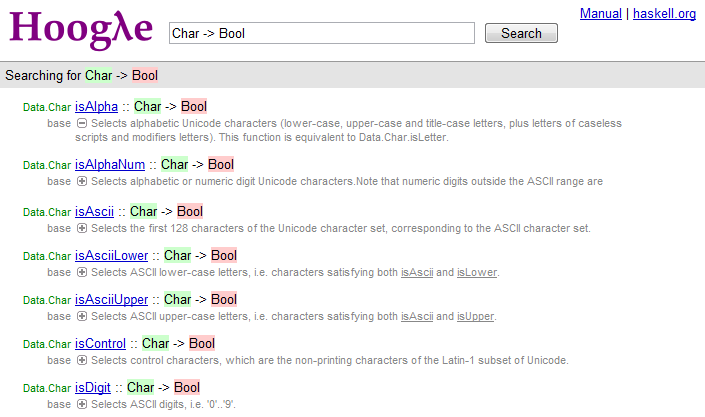
\includegraphics[width=\textwidth]{web.png}\fi
\caption{Hoogle web use.}
\label{fig:web}
\end{figure}

\begin{figure}
\ifpdf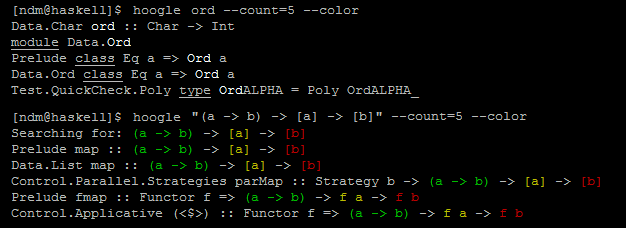
\includegraphics[width=\textwidth]{cmdline.png}\fi
\caption{Hoogle command line use.}
\label{fig:cmdline}
\end{figure}

There are three main methods of using Hoogle:

\begin{description}
\item[Web Interface] The web interface is just like a normal web search engine, requiring no special software or installation. Just visit the website and enter your search terms. An example of the web interface is shown in Figure \ref{fig:web}. \\
    URL: \textsf{http://haskell.org/hoogle/}
\item[Command Line] The command line tool can be downloaded from Hackage \cite{hackage}, and installed using the standard Cabal commands \cite{cabal}. The command line tool has more options, and allows searches to be performed while offline. An example session is shown in Figure \ref{fig:cmdline}. \\
    URL: \textsf{http://hackage.haskell.org/cgi-bin/hackage-scripts/package/hoogle}
\item[Lambdabot Interface] When using Lambdabot \cite{lambdabot}, you can invoke the Hoogle plugin with \texttt{@hoogle}.
\end{description}


\section{Version History}

Hoogle is now over four years old, and has undergone four complete rewrites. This section describes each version.

\subsection{Hoogle 1}

I started work on the original version of Hoogle before I started my PhD, with only basic Haskell knowledge, and long before I had ever encountered a Monad. Realising that my PhD was likely to be dominated by Haskell, I decided to develop a tool to help beginners (such as myself) find some of the useful functions located in the standard libraries. While learning Haskell I had watched experienced programmers take my code and simplify it significantly, by using some clever function whose existence I was unaware of. I wanted to perform the same tricks!

The initial version of Hoogle was web based, and relied on client-side Javascript to perform searches. The use of Javascript was unavoidable for a client-side web program, but even with my limited Haskell experience I longed for proper algebraic data types, pattern-matching and type-safety. The list of functions was obtained from the ZVON Haskell Reference \cite{zvon}, who kindly provided all their function data in XML, for anyone to use. Hoogle worked, but suffered from huge page load times (it had to transfer 8MB of data), and wasn't particularly easy to use.

\subsection{Hoogle 2}

Once I started my PhD I was exposed to lots of Haskell, and decided to rewrite Hoogle in Haskell. Originally version 2 was a direct port of version 1 to Haskell, with the searching logic moved to a server-side CGI program. However, once Hoogle was written in Haskell it became much easier to explore type searching, treating types as algebraic data structures. As soon as version 2 was placed on the web, members of the \verb"#haskell" IRC channel \cite{irc} began to use and discuss it. The feedback and encouragement provided by \verb"#haskell" resulted in many improvements.

Version 2 was my first real experience at programming a large Haskell project, and it showed. The code was poorly organised. The parser could easily be crashed by entering malformed searches. Many features were littered throughout the code, without clear isolation. Much of the code failed to make use of the standard functional idioms. Eventually I reached the stage where every improvement became an increasingly large amount of work, and became more likely to conflict with an existing feature.

\subsection{Hoogle 3}

The goal of version 3 was to improve the code so that features could be added easily. Hoogle 3 was always intended to be the definitive version, which would be modified, but never rewritten from scratch. The ZVON function list was replaced with information extracted from Haddock \cite{haddock}, which allowed all of the hierarchical libraries to be searched. The experience of writing version 2 provided many insights, which were incorporated. A log of all the searches performed was used to determine where Hoogle didn't match the users expectations. The end result was a more polished tool.

However, version 3 was still insufficient in many ways -- the most obvious design flaw was the inability to search for higher-kinded type classes, of which \code{Monad} is by far the most common. The other problem was scalability, Hoogle 3 scaled linearly in the number of functions available, which worked fine on a small function database, but became a problem when attempting to search more libraries.

\subsection{Hoogle 4}

After submitting my PhD, I spent the summer working on Hoogle, sponsored by the Google Summer of Code. Once again, version 4 was a complete rewrite. The largest change is that instead of using a text file containing a list of functions, version 4 uses a binary database. This change allows Hoogle to perform searches faster, and to scale better as more functions are added to the database.

By storing some precomputed information, searches can be made faster. For example, if the database included the answer for all queries of length 5 and below, these searches could be answered very quickly. However, the database would also grow unacceptably large. Version 4 required many trade-offs, choosing the right representation to maximise search speed and minimise database size. For example, text searching in version 3 has time complexity $O(m \cdot n)$, where $n$ is the number of functions and $m$ is average length of a function name. Early releases of version 4 used a trie and required only $O(m)$ to find all the results, but at the cost of a large database. The current version requires $O(m \cdot \log n)$ to find the answers which match the prefix of the search, then uses heuristics to find additional answers quickly -- although with a time complexity of $O(m \cdot n)$.


\section{The Future}

I hope that version 4 will be the last ever rewrite of Hoogle. Now there is a stable base to work from, the hope is that additional features can be added neatly. Some of the planned features are given in this section, but none have any timescale given.

\subsection{Index Hackage}

Hoogle currently doesn't index all the packages available on Hackage, but it should. The work done for version 4 has enabled Hoogle to scale to the necessary number of packages, so hopefully Hoogle requires no changes. However, before a package can be indexed by Hoogle it must have documentation generated by Haddock, and this has proved a stumbling block. To install all of Hackage is a challenge, and to do so on my ailing Windows machine is an impossibility. Hackage already generates Haddock documentation for all packages, and once this process has been revamped, hopefully Hoogle information can be generated at the same time.

\subsection{Hoogle Local}

Hoogle Local is a graphical user interface to Hoogle, giving the same interface as the web version, but operating offline. Hoogle Local allows users to locally install API databases, customise Hoogle to a greater degree, and doesn't require an internet connection -- but provides the same user friendly interface as the web version. This feature has been partially implemented, making use of Firefox 3 as an XULRunner host. The development version is useable but lacks the necessary polish to release more widely.

\subsection{Multilingual Hoogle}

Hoogle is currently focused on Haskell, with support for most GHC type system extensions. But internally, Hoogle does not support all of Haskell's advanced type features -- multi-parameter type classes are not supported directly, but are translated into single-parameter type classes. A more accurate description might be that Hoogle supports searching over a core type language, which Haskell's type language is translated into. We suspect that other programming languages could also be translated into Hoogle's type system. There are three classes of programming languages that Hoogle might support:

\begin{itemize}
\item Languages based on the Hindley-Milner type system. Some of these languages have type systems which are a subset of Haskell. These languages should permit a fairly straightforward translation -- obvious examples include ML and Clean.
\item Strongly typed languages, typically object orientated. F\# has shown that a functional language can interface with object-orientated languages in a reasonably natural way, by adding some features and by translating others. Hoogle could use some of the same ideas, and expand to search languages such as Java and C\#.
\item Untyped languages, typically scripting languages. Languages such as Perl, Python and Javascript don't have any formal types in their interfaces, but often there is some notion of what subset of values should be passed to which function -- sometimes encoded as a runtime check. This information could be used to give approximate types to functions, and allow Hoogle searching.
\end{itemize}

Hopefully one day Hoogle will be a general purpose programming language search engine, that works well for both Haskell and other programming languages.

\section{Design Guidelines}

This section explains the guidelines used for organising the Hoogle codebase. This information is intended to serve both as a reference to budding Hoogle developers, and as my current view of best practices in large-scale Haskell development. Hoogle has been rewritten from scratch four times, each time incorporating knowledge gained from previous attempts, and iteratively improving the code layout. Some of these lessons may apply to other projects, and help avoid painful rewrites!

\subsection{Structure your code as a library}

Hoogle is a program, but is structured as a library, with client programs which make use of the library. Anything in the \code{Hoogle.*} module tree is part of the library, and is carefully checked to expose a sensible interface. Each client which makes use of Hoogle has its own top-level module. For the purposes of deployment, there is no library, but if the need arises an explicit library can easily be added. By forcing a split between the underlying functionality and the user interface, and by imagining other potential users of the library, we gain a cleaner separation of concerns.

\subsection{Put types in their own module}

All the data type definitions are placed in a module of their own, at the bottom of the import hierarchy. For example, type signatures are defined in the module \code{Hoogle.TypeSig.Type}. This module also contains basic utility functions (\code{isTypeApp}, \code{fromTypeApp}) and instances (\code{Eq}, \code{Show}). I have found that by separating out data type definitions, it is much easier to avoid mutual recursion between modules.

\subsection{Group operations on a type}

All basic operations on a type share the same module prefix. For example, operations on type signatures are given module names such as \code{Hoogle.TypeSig.Parse} and \code{Hoogle.TypeSig.Render}, each responsible for one particular operation. For modules wishing to use type signatures there is \code{Hoogle.TypeSig.All} which imports and reexports \code{Hoogle.TypeSig.*}, usually with a more restrictive export list. The intention is that no module outside of \code{Hoogle.TypeSig} should ever import a module other than \code{.All}. Many internal details can be hidden from the users of type signatures, which are useful to expose to the operations on type signatures.

Originally the \code{.All} module was simply called \code{Hoogle.TypeSig} -- which seems like a more natural choice. However, having the \code{.All} module in the same directory as the other related modules is beneficial, and makes it easier to keep the modules in sync. Additionally, it becomes easy to spot when a module from a different module prefix imports something in violation of the guidelines.

\subsection{Use a hierarchy}

Hoogle is structured as a library, with \code{Hoogle.All} exporting all the definitions that a client may wish to use. Anything exported from this module is intended as a permanent interface, and is relatively stable. Unfortunately, often clients of the Hoogle library need access to more specific details -- details that are semi-stable, but which are not ready to form part of the standard interface. By letting clients import modules such as \code{Hoogle.TypeSig.All}, the official interface avoids getting polluted, but the features can be still implemented.

Over time I hope that clients importing modules other than \code{Hoogle.All} will decrease, as proper thought is given to the interface, and the right abstractions are identified. By allowing greater flexibility the hope is that long-term maintenance will not be hampered by the pressing need to add one particular feature.

\subsection{Provide one executable}

Version 3 had four executable programs -- one to generate ranking information, one to do command line searching, one to do web searching, and one to do regression testing. Version 4 has one executable, which does all the above and more, controlled by flags. There are many advantages to providing only one end program -- it reduces the chance of code breaking without noticing it, it makes the total file size smaller by not duplicating the Haskell run-time system, it decreases the number of commands users need to learn. The move to one multipurpose executable seems to be a common theme, which tools such as darcs and hpc both being based on one command with multiple modes.

\section{Conclusion}

Hoogle has benefited greatly from feedback, encouragement, technical contributions, bug reporting and more. Versions 2 and 3 were helped substantially by many members of the functional programming group at York University, and the users of \verb"#haskell". While writing version 4 I was mentored by Niklas Broberg, received lots of help from Duncan Coutts, and was funded by Google through the haskell.org project. Hoogle has benefited from substantial contributions from David Waern, Don Stewart, Esa Ilari Vuokko, Gaal Yahas, Ganesh Sittampalam, Gwern Branwen, Henk-Jan van Tuyl, Mike Dodds, Thomas Davie, Thomas J\"{a}ger, Tillmann Rendel and Udo Stenzel.

Hoogle is not finished. In addition to the future tasks given in this article, there are plenty of suggestions and bugs outstanding, most of which are documented in the bug database (\textsf{http://code.google.com/p/ndmitchell/issues/list}). Some bugs are marked as beginner, meaning they can be easily tackled by someone new to Hoogle -- and in some cases someone new to Haskell. If anyone wants to help, please email me at \textsf{ndmitchell@gmail.com}.

As the task of programming goes from one of painting on a blank canvas, to one of plumbing together existing components, Haskell has a distinct advantage with its high-level abstractions. As the number of libraries increases, finding the right functionality becomes harder. Hoogle aims to help by providing a simple way to find the right functions.


\bibliography{hoogle}

\end{document}
